\documentclass[nocopyrightspace]{acm_proc_article-sp}
\usepackage{amsmath}
\usepackage{amsfonts}
\usepackage{amssymb}
\usepackage[algoruled]{algorithm2e}
\usepackage{tabularx}

%Remove the box from the bottom left from the template
\makeatletter
\def\@copyrightspace{\relax}
\makeatother
\hyphenation{IterSampLP}
\hyphenation{SampLP}

\begin{document}

\title{Randomized Linear Programming}
\subtitle{Lab Report Randomized Algorithms IN4337}
\numberofauthors{2} 
\author{
\alignauthor
Koos van der Linden \\ \affaddr{4133145}
% 2nd. author
\alignauthor
Marieke van der Tuin \\ \affaddr{4079299}
}
\maketitle
\begin{abstract}
For linear programming problem instances that have a relative small dimension compared to the number of constraints, two randomized algorithms, SampLP and IterSampLP, are compared in runtime and asymptotic bounds with Simplex, a deterministic algorithm. It is shown that SampLP performs better than Simplex on instances with small dimension. This is not shown for IterSampLP. By analyzing the asymptotic bounds it is expected that IterSampLP will perform better than both SampLP and Simplex when the number of constraints is much larger and the dimension is still relatively small.
\end{abstract}

\section{Problem introduction}
The Linear programming problem is concerned with finding the optimum of an objective function limited to a set of constraints. The standard form of a linear program is written in equation \ref{eq:standard}, with $x$ the vector variables to be determined and $A$ the matrix of constraints that should be less or equal to vector $b$.
\begin{equation}
\label{eq:standard}
\begin{split}
\text{minimize } & \mathbf{c}^T \mathbf{x} \\
\text{subject to } &  \mathbf{Ax} = \mathbf{b} \\
\text{and } & \mathbf{x} \geq \mathbf{0}
\end{split}
\end{equation}

with $\mathbf{x}$ the vector variables to be determined and $\mathbf{A}$ the matrix of constraints that should be equal to vector $\mathbf{b}$. If the constraints are in the form $\mathbf{a}^T \mathbf{x} \leq b$ or $\mathbf{a}^T \mathbf{x} \geq b$, slack variables can be introduced to rewrite the problem to the standard form. 

In this report, three algorithms that solve linear programming problems are examined: Simplex, SampLP and  \\ IterSampLP. The last two of these are randomized algorithms. Simplex is the oldest of these algorithms. This algorithm uses the standard form as an input and has a time complexity of polynomial time on average, but has a worst-case complexity of exponential time. How do SampLP and IterSampLP compare with this? It is expected that these algorithms will perform better on instances with small dimension (the number of variables) and large number of constraints. Examples of problems with relatively small dimension are the smallest enclosing circle problem and the weighted Euclidian one-center problem

\section{Description of used methods}
Three methods are compared  in this report: Simplex, the only deterministic method, and SampLP, a recursive randomized algorithm, and IterSampLP, an iterative randomized algorithm.
\subsection{Simplex}
The Simplex algorithm \cite{dantzig1951maximization} is the most basic algorithm for solving linear programming problems. This algorithm uses the standard form as an input and has a time complexity of polynomial time on average, but has a worst-case complexity of exponential time. This methods works as follows: \\
The set of constraints $H$ (defined by $\mathbf{Ax} \leq \mathbf{b}$), and the constraint that all variables should be non-negative ($x \geq 0$), define a feasible region. This feasible region is a polytope. In the case of 2 dimensions ($d=2$), this can be easily seen: all area within the lines defined by $H$ and the axes is called the feasible region. \\
The algorithm can be split in two phases. In phase I, the feasible region is defined, and an initial solution is found (or the algorithm returns because the problem is infeasible. This is the case when the feasible region is empty). In phase II, the program travels along the edges of the feasible region in the direction that minimizes the objective function. It stops when the optimum is found.

The steps for solving an LP instance in standard form are as follows. First a so called tableau is formed, in which the first row is the objective function, and the other rows are the constraints:
\[
\begin{bmatrix}
1 & -\mathbf{c}^T & 0 \\
0 & \mathbf{A} & \mathbf{b}
\end{bmatrix} \]

In each iteration, one column and row in $A$ is chosen with a non-zero pivot. This row is multiplied so that this pivot becomes one. Then this row is subtracted from all other rows. The result is that all elements in the pivot column (except the pivot itself) become zeros. This pivot-row is chosen in such a way to minimize $Z$, ($Z = \mathbf{c}^T \mathbf{x}$), the top right element in the tableau)). As soon as all elements in the first row are negative, an optimal solution is found. The top right element of the transformed tableau contains the minimum value. \\
The values of the variables is determined as follows: with the final tableau, discern basic and non-basic variables. In the final objective function, non-basic variables have a non-zero factor, and the basic variables have a zero factor. The value of all non-basic variables are zero. For the basic variables: find the row with the only $1$ in the column (the rest is all zero's). The last element in this row (in the transformed $\mathbf{b}$ vector, is the value for this basic variable.

In \cite{spielman2004smoothed} the runtime of Simplex is analysed extensively. But the authors admit that their understanding of the simplex algorithm is far from complete. It is shown that the average runtime is polynomial, but the runtime depends for a large part on the choice of pivot-rule.  Until now, for every deterministic pivot rule a counter example has been found that can only be solved in exponential time, so the worst case running time is exponential.
                         

\subsection{Simplex implementations}
For testing purposes, two implementations of Simplex were used: Gurobi, and Apache. The Gurobi optimizer is a commercial solver for linear programming problems. It gives several interfaces to use the solver, including Java. With Apache, the Simplex Solver that is included in the open source library of Apache Software Foundation, is meant.\\
Gurobi is used to determine the feasibility of randomly generated linear programming instances. Apache is used to compare the run time with the two randomized algorithms. Apache is also used in these algorithms, when Simplex is called.

\subsection{SampLP}
The SampLP algorithm (\ref{alg:samplp}) was introduced by Clarkson\cite{clarkson1988vegas}. This randomized Las Vegas algorithm only gives a speed-up for instances with a small dimension. Examples of these type of instances is the smallest enclosing circle problem and a Chebyshev approximation. For instances with a larger dimension ($n>9d^2$), the Simplex algorithm is called directly.

The algorithm first selects a random subset of constraints and then recursively calls itself. If the set of constraints is getting small, the Simplex algorithm is called, resulting in an optimal solution. The output vector $x$ of the recursive call is afterwards checked by looking whether it is violating any of the constraints. If no violations are found any more, the solution vector $x$ is correct and is returned. 

\begin{algorithm}[h]
\label{alg:samplp}
\caption{SampLP}
\KwIn{A set of constraints $H$}
\KwOut{The optimum $\beta(H)$}
$S \gets \phi$\;
\If{$n<9d^2$}{
	\Return{Simplex($H$)}\;
}
\Else{
	$V \gets H$, $S \gets \phi$ \;
	\While{$|V| > 0$}{
		Choose $R\subset H\setminus S$ at random, with $|R| = r = min\{d\sqrt{n},|H\setminus S|\}$ \;
		$x \gets SampLP(R\cup S)$ \;
		$V \gets \{h \in H|$vertex defined by $x$ violates $h\}$\;
		\If{$|V|\leq 2 \sqrt{n}$}{
			$S \gets S \cup V$ \;
		}		
	}
	\Return{$x$}\;
}
\end{algorithm}

The set $V$ of constraints that violate $H$ is small: it is expected that it contains  $\frac{d(m-r+1)}{r-d}$ constraints. Using the Markov inequality this results in $Pr[|V|>2\sqrt{n}]\leq \frac{1}{2}$. Therefore, the while loop has an expected number of iterations of maximum 2. The set $S$ gets in each of the $d$ phases at most $2\sqrt{n}$ constraints. Therefore, the set $R \cup S$  never exceeds the size of $3d\sqrt{n}$. Checking the possible violation of constraints takes $O(d^2n)$. This results in a bound of $T(n) \leq 2dT(3d\sqrt{n})+O(d^2n)$, for $n>9d^2$. 

If $n<9d^2$ the simplex algorithm is called. This takes  $O(d)^{d/2+O(1)}$. 

In total, this results into a complexity bound of
\begin{equation}
O(d^2n)+\log{\frac{n}{d^2}}^{\log{d+2}}O(d)^{d/2+O(1)}
\end{equation}

\subsection{IterSampLP}
The more sophisticated IterSampLP algorithm (\ref{alg:itersamplp}) was also introduced by Clarkson\cite{clarkson1995vegas}. It is also an algorithm which only gives a speed-up if the number of variables is small: if $n<9d^2$ the Simplex algorithm is called. The iterative IterSampLP uses weighted constraints. For each step it selects a random subset of constraints of size $9d^2$. Next, the Simplex algorithm is called using these values. The result of the Simplex call is used to reweigh the constraints that violate $x$. A constraint with a higher weight has a higher probability to be selected in the next random choosen set. 

\begin{algorithm}[h]
\label{alg:itersamplp}
\caption{IterSampLP}
\KwIn{A set of constraints $H$}
\KwOut{The optimum $\beta(H)$}
$\forall h \in H, w_h \gets 1$ \;
\If{$n<9d^2$}{
	\Return{Simplex($H$)}\;
}
\Else{
	$V \gets H$ \;
	\While{$|V| > 0$}{
		Choose $R\subset H$ at random, with $|R| = r = 9d^2$ \;
		$x \gets Simplex(R)$ \;
		$V \gets \{h \in H|$vertex defined by $x$ violates $h\}$\;
		\If{$\displaystyle\sum_{h\in V} w_h \leq (2 \displaystyle\sum_{h \in H} w_h)/(9d-1)$} {
			$\forall h \in V, w_h \gets 2w_h$ \;
		}		
	}
	\Return{$x$}\;
}
\end{algorithm}

The expected number of iterations of the while loop is \\ $O(d log(n))$, since the total weight of minimum required constraints grows much faster than the total weight of all constraints, since they are more likely to violate result vector $x$. In the while loop the simplex algorithm is called. This takes $O(d)^{d/2+O(1)}$. Checking the violating constraints takes $O(dn)$. 

This results in a complexity bound of:
\begin{equation}
O(d^2n \log{n}) + d \log{n} O(d)^{d/2+O(1)}
\end{equation}
\vfill
\section{Experimental results}
%benchmark miplib: which instances to choose?
To test the performance of the Linear Programming algorithms, two different methods are used: by using benchmarks and by generating random graphs.

First of all, the Simplex implementation of Apache is tested by using the benchmark MIPLIB 2010 \cite{KochEtAl2011}. This benchmark has Mixed Integer Problems. We are only considering continuous problems. Luckily, next to the integer objective also the LP (continuous) objective is provided for each problem instance. The Gurobi implementation is assumed to be correct and was previously tested by others using the MIPLIB benchmark. The runtime results for SimplexApache on instances of MIPLIB can be seen in table \ref{tab:miplibresults} in the appendix and in figure \ref{fig:miplibresults_n} and \ref{fig:miplibresults_d}. Since the benchmark instances are very large and therefore require lots of time to test, only a small subset of the benchmark is used to test the performance of SimplexApache. The choice of this subset was based upon problem size and alphabetic order. Next to recording the required time, the solutions were also checked for correctness. This was the case for all problem instances. 

\begin{figure}[h!]
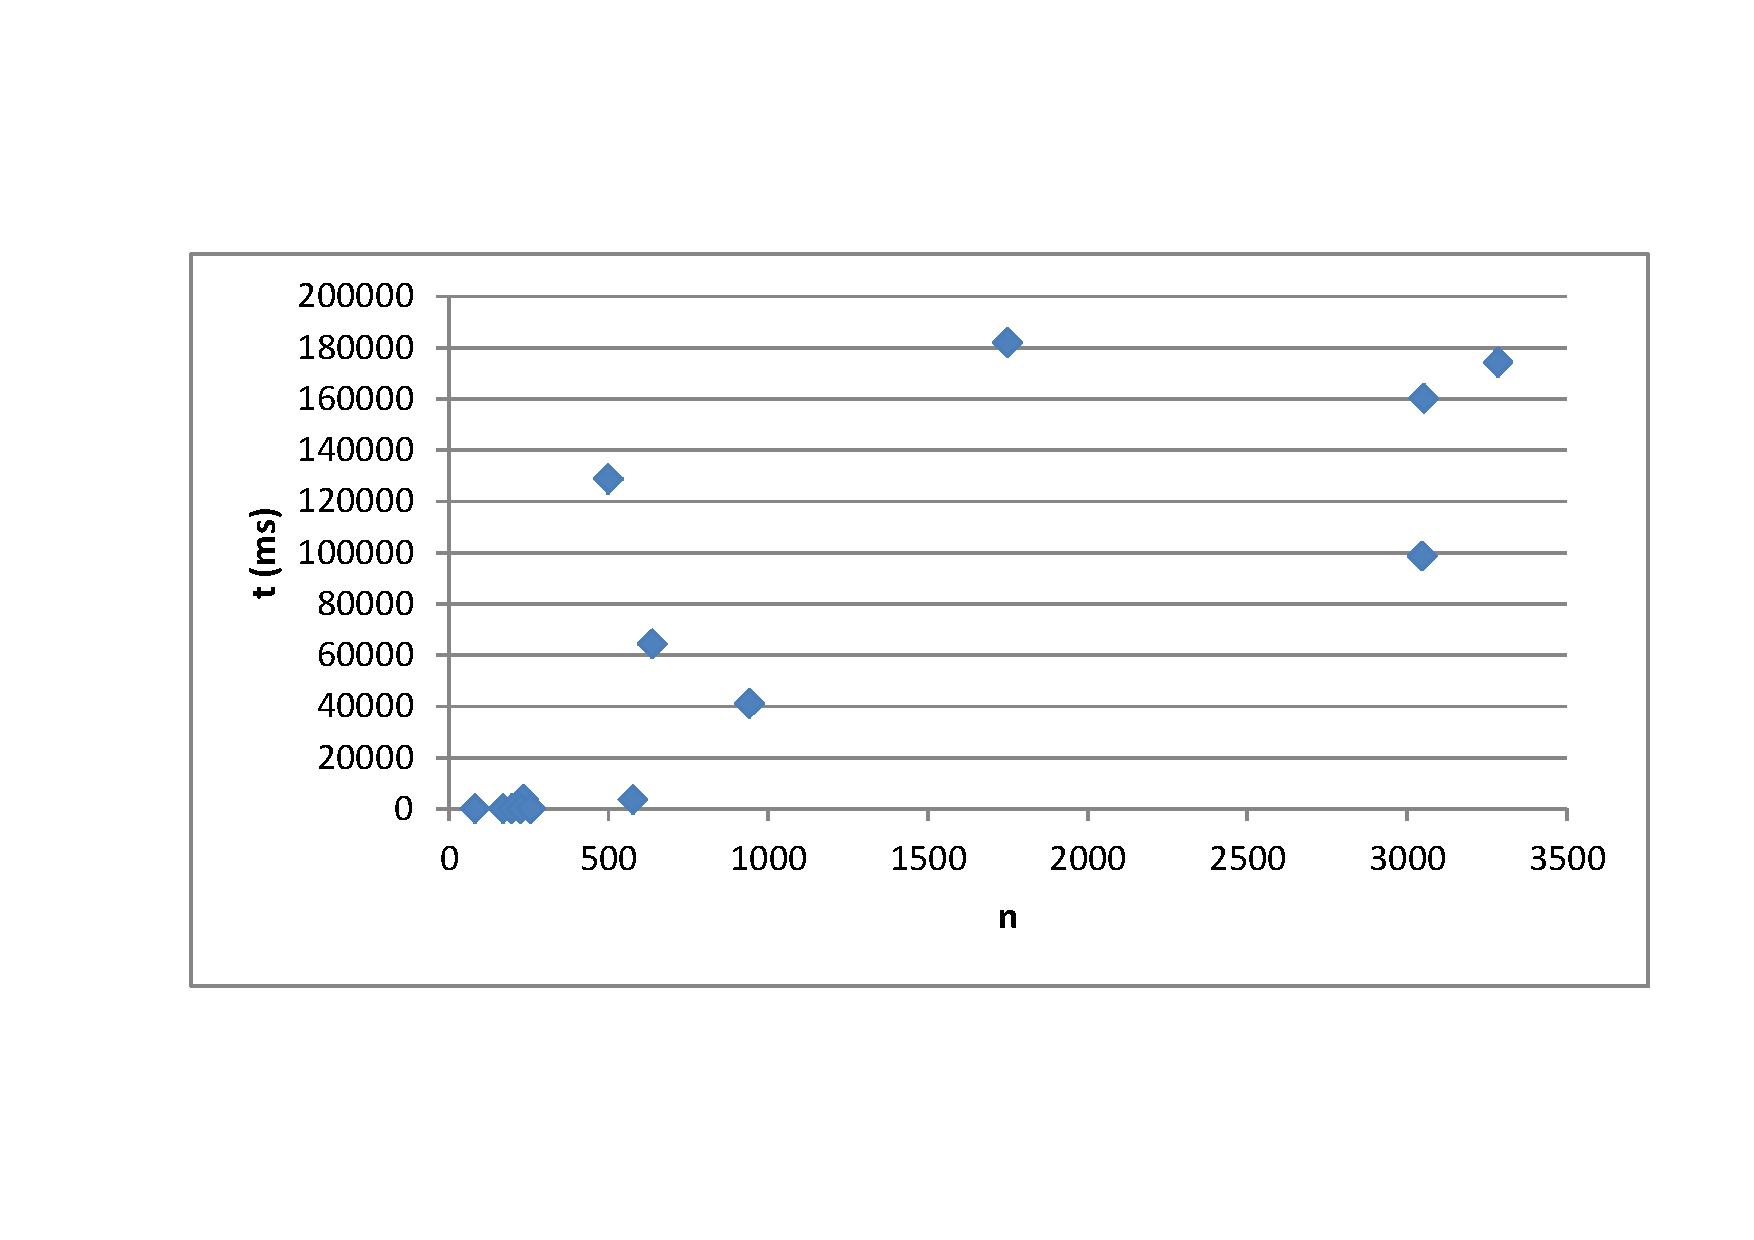
\includegraphics[width=\columnwidth]{../Results/miplib_apache_n.pdf}
\caption{Runtime results for SimplexApache on instances of MIPLIB 2010 \cite{KochEtAl2011} compared to the number of constraints: $n$}
\label{fig:miplibresults_n}
\end{figure}
\begin{figure}[h!]
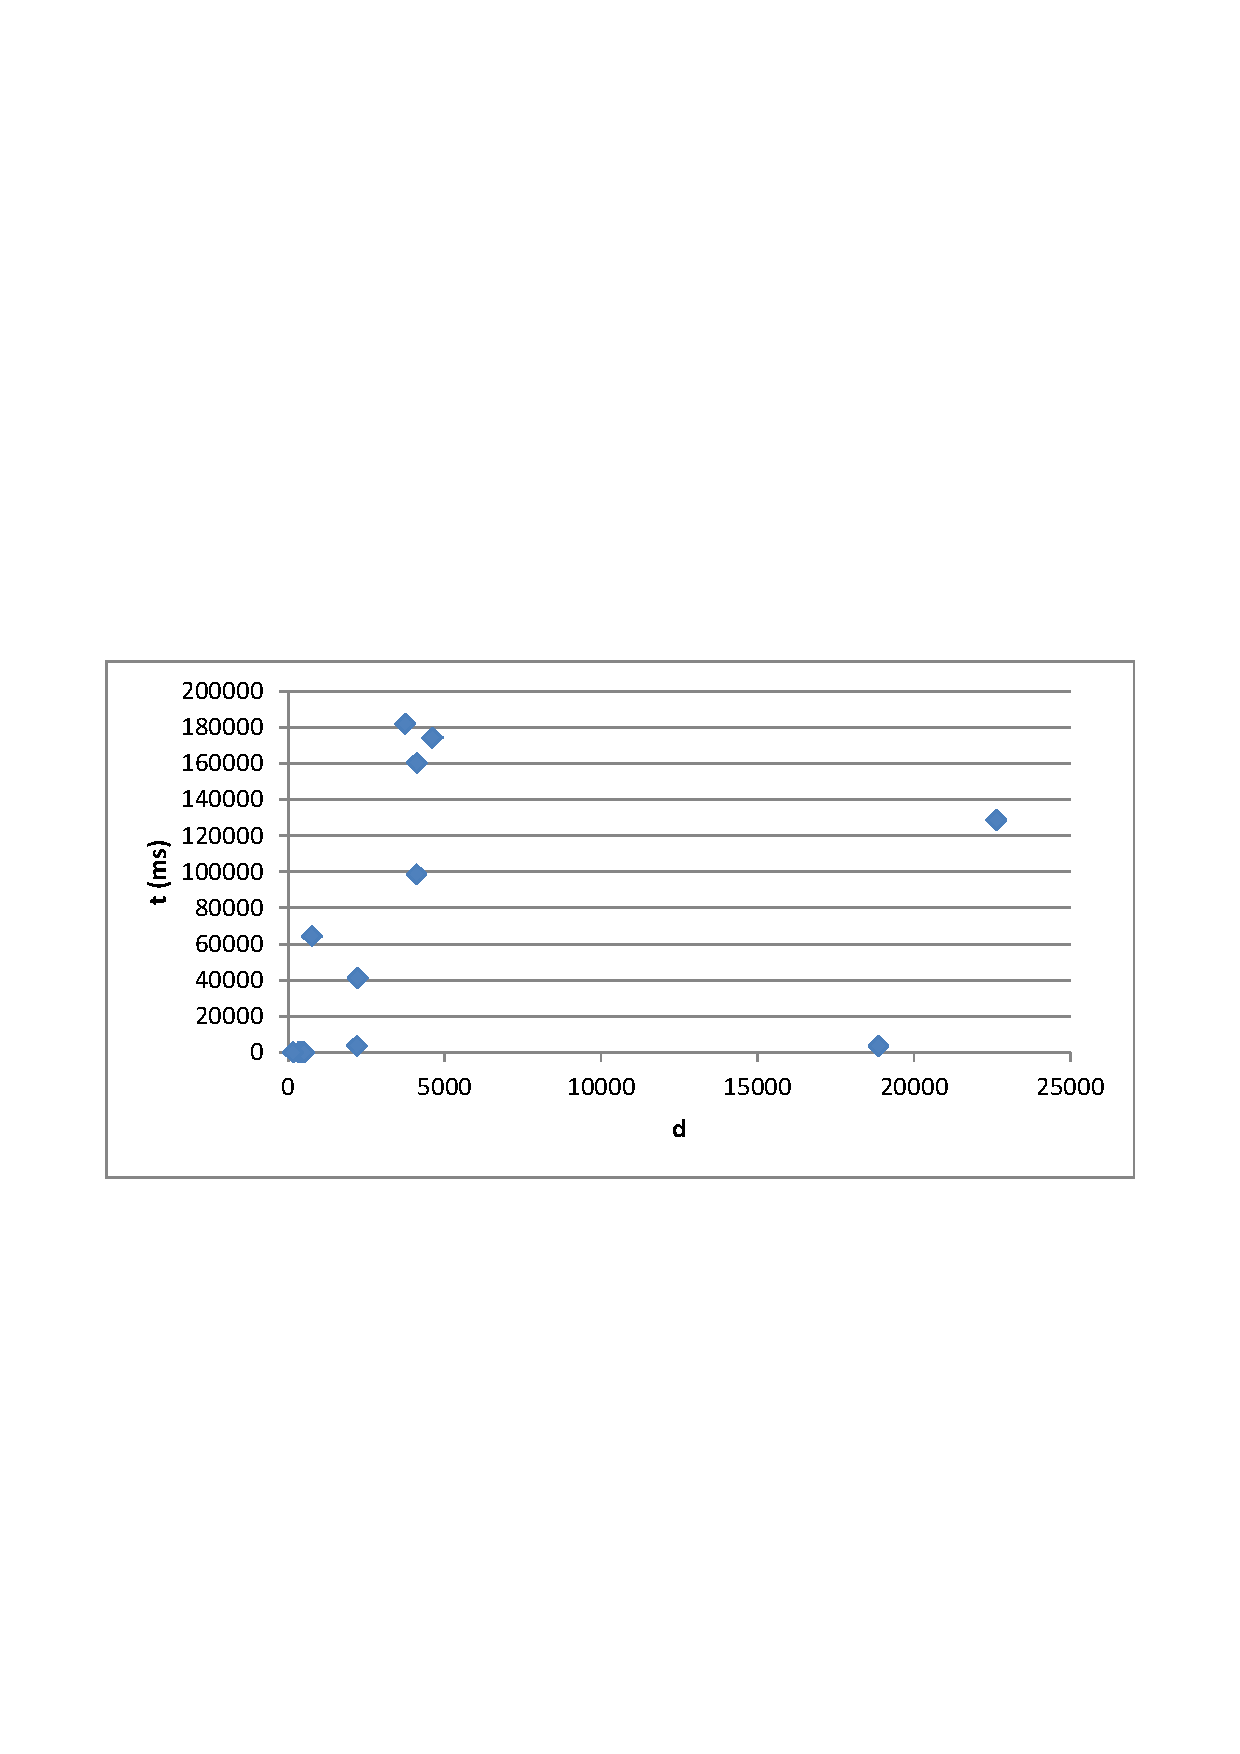
\includegraphics[width=\columnwidth]{../Results/miplib_apache_d.pdf}
\caption{Runtime results for SimplexApache on instances of MIPLIB 2010 \cite{KochEtAl2011} compared to the number of variables: $d$}
\label{fig:miplibresults_d}
\end{figure}

Unfortunately, this benchmark could not be used to test the performance of SampLP and IterSampLP, because for all instances in this benchmark $n < 9d^2$. 

Therefore, to test the performance of the randomized algorithms, a linear programming problem generator is used. This generator generates problems with uniformly random constraints and a random objective function. The feasibility of each generated problem is tested with Gurobi, and feasible instances are stored for later use.

%aantal iteraties binnen simplexApache voor sampleLP & iterSampLP
With the generator first a set of feasible problem instances was randomly generated, with $d$ ranging from $2$ to $9$, and with $n = 10d^3$, so $n > 9d^2$ always holds. For each value of $d$, four linear programming problems were generated. 

Next, the algorithms are run given these problem instances. Each algorithm was repeated $100$ times for each problem instance and the results were used to calculate an average runtime. Runtime is measured in two ways: the total runtime and the Simplex runtime. The Simplex runtime is defined as the time the SimplexApache algorithm is run in total. SampLP and IterSampLP both call Simplex for small instances of the original problem. By measuring the time Simplex is running, a comparison can be made that is less dependent on the implementation of SampLP and IterSampLP.

The results can be seen in table \ref{tab:relativeresults} and the corresponding figures \ref{fig:totalruntime}, \ref{fig:simplexruntime} and \ref{fig:simplexruntime_relative_simplex}. In the figures, the runtime is only compared with $n$, the number of constraints and no longer with $d$. This is because $n$ depends on $d$ ($n=10d^3$). 

\begin{figure}[h!]
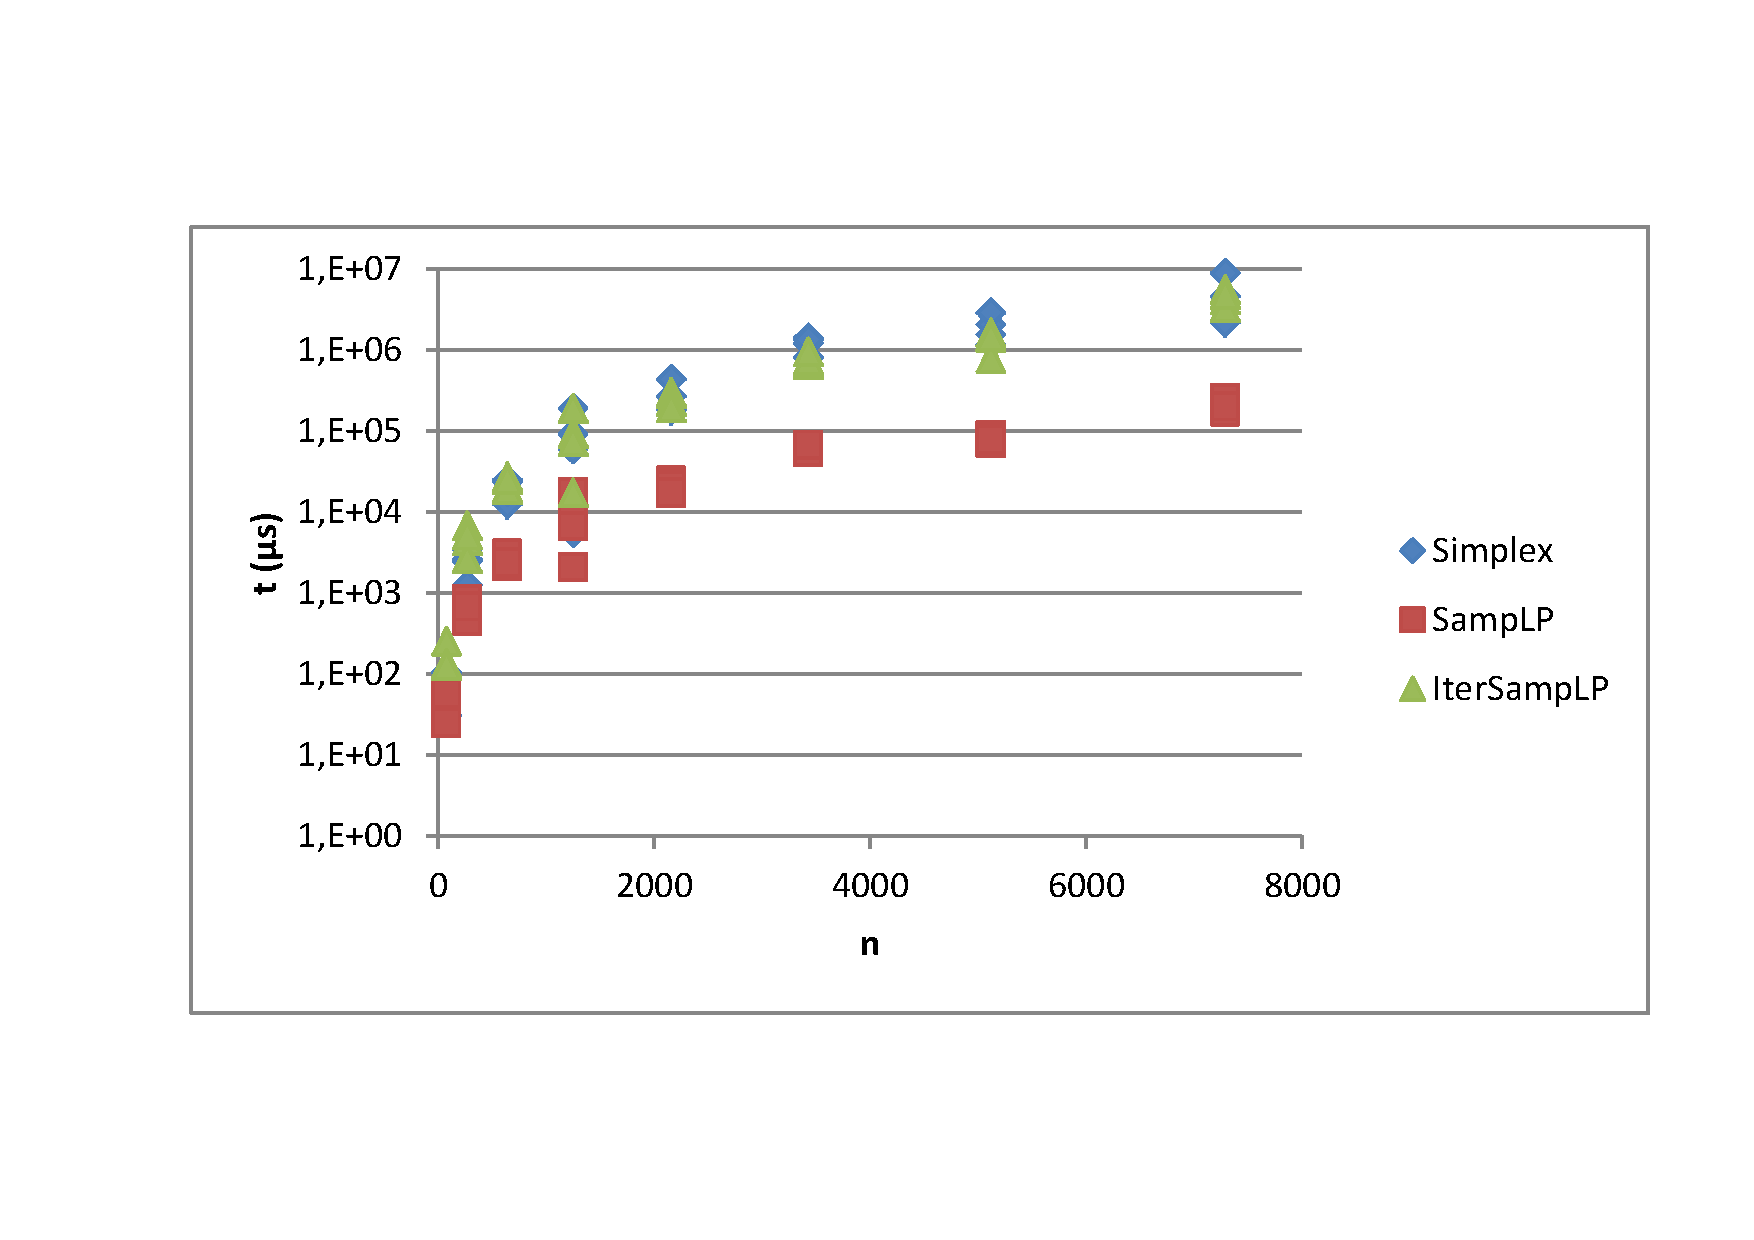
\includegraphics[width=\columnwidth]{../Results/totalruntime.pdf}
\caption{Runtime results for SimplexApache, SampLP and IterSampLP on the randomly generated problems. The total runtime is measured.}
\label{fig:totalruntime}
\end{figure}

\begin{figure}[h!]
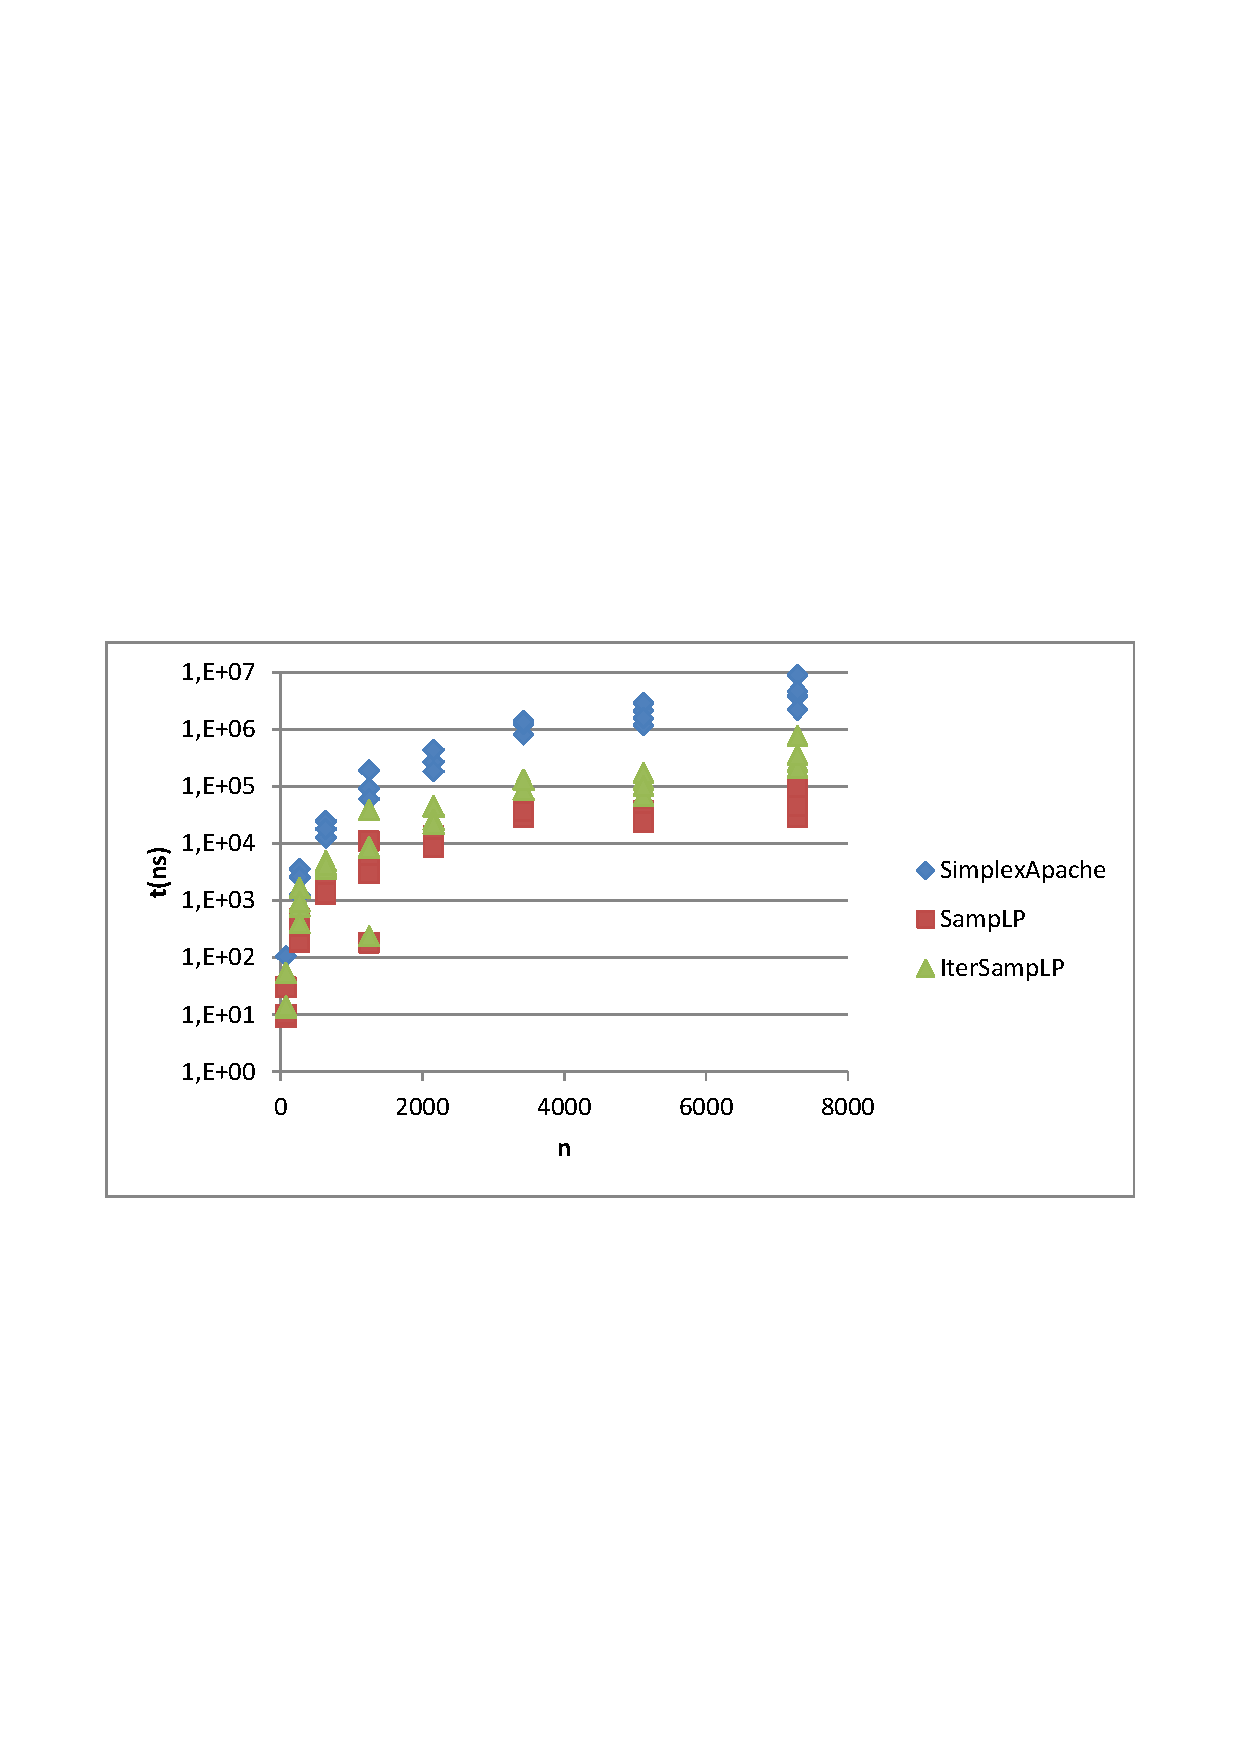
\includegraphics[width=\columnwidth]{../Results/runtime_Simplex.pdf}
\caption{Runtime results for SimplexApache, SampLP and IterSampLP on the randomly generated problems. Only the time Simplex is running is measured.}
\label{fig:simplexruntime}
\end{figure}

\begin{figure}[h!]
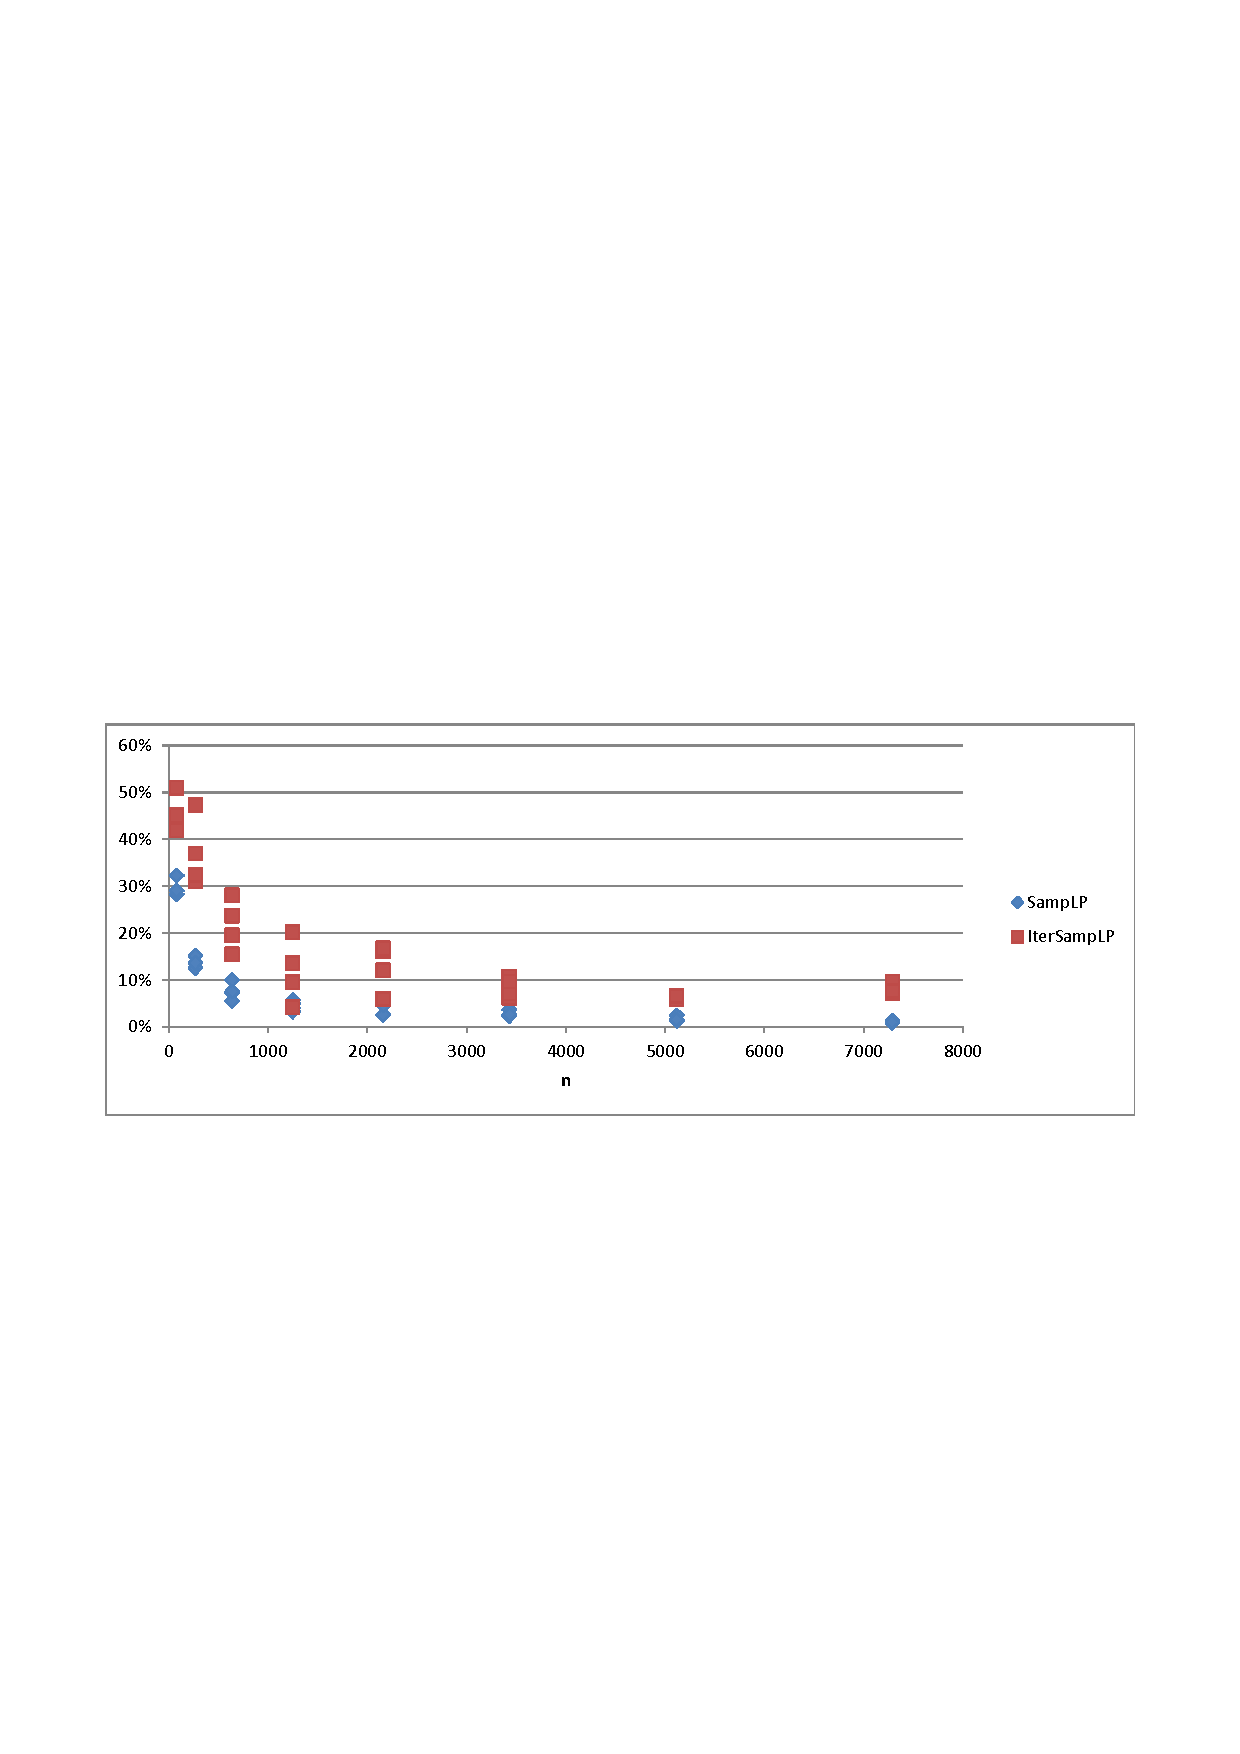
\includegraphics[width=\columnwidth]{../Results/simplexruntime_relative_simplex.pdf}
\caption{Runtime results for SampLP and IterSampLP on the randomly generated problems. Only the time Simplex is running is measured. The runtime of SampLP and IterSampLP is plotted against the runtime of SimplexApache as a percentage.}
\label{fig:simplexruntime_relative_simplex}
\end{figure}
\vfill
\section{Analysis of results}
From figure \ref{fig:miplibresults_n} it can be concluded that the Simplex runtime is generally higher for a larger number of constraints. The relation between $n$ and the required time seems to be quite polynomial, as was expected from the runtime analysis of Simplex. 

However, the plot showing the dimension against the time (Figure \ref{fig:miplibresults_d}) doesn't exactly seem to follow this polynomial bound. For values of $d$ smaller than 5000 it somewhat holds, but for the 2 larger values of $d$ in the considered benchmark ($d=18866$ and $d=22641$), this relation doesn't hold: the running time is much lower than you would expect if there really is a polynomial relationship. It might be the case that - besides values for $d$ and $n$ instances can be marked "easy" or "difficult", for example depending on the number of zeros in the matrix $A$ and the maximum and minimum values.

In figure \ref{fig:totalruntime} the runtime of the SimplexApache, SampLP and IterSampLP is considered for our own generated instances. Plotted on a logscale, it can be concluded that the SimplexApache implementation does not behave polynomially on average for our examples. The SampLP and IterSampLP do correctly show their logarithmic complexity bounds. SampLP always runs faster than Simplex. \\ IterSampLP sometimes is faster than Simplex, but sometimes is not. 

The runtime was also considered by the time the Simplex algorithm was running. These results are shown in figure \ref{fig:simplexruntime} and \ref{fig:simplexruntime_relative_simplex}. It can be seen that the SampLP algorithm only requires $8\%$ of the Simplex running time on average compared to Simplex Apache. \\ IterSampLP requires a bit more Simplex time ($19\%$), since it is called in every iterative step to compute the optimal solution of the random subset. Compared with figure \ref{fig:totalruntime} it can be seen that IterSampLP should have a lot of time consuming operations next to calling the Simplex algorithm. This is indeed the case: reweighting after each step takes quite some time. A more efficient implementation of this reweighting process might cause a better performance of IterSampLP in general. 

SampLP performs in our experiments better than IterSampLP. This is as expected if you look into the runtime analysis. For instances with larger values for $n$, IterSampLP theoretically should perform better than SampLP. However, these instances are such large that they are not runnable on a simple machine without generating Out Of Memory or Heap Space errors.

\section{Discussion of the benefit of randomization for the problem}
It has been shown that SampLP gives an enormous speed-up compared to the Apache Simplex implementation. \\ IterSampLP sometimes does this, but is expected to do so for large problem instances. It is therefore useful to use the randomized versions. However, the presented randomized algorithms do not work for all instances. It only gives a speed-up if $n>9d^2$. Else, the Simplex algorithm is called immediately. This requires very specific problem instances with small dimensions. The smallest enclosing circle problems are for example perfectly solvable with randomized algorithms, since these always have a dimension of 3.

Although randomized algorithms provide a speed-up, a professional LP solver like Gurobi still performs better for instances with a large $n$. The randomized algorithms might be improved by using the Gurobi solver instead of calling the Simplex algorithm. For larger $n$ this should give a speed-up, since the Gurobi solver should be more optimized than a general Simplex optimization. If then the runtime of the randomized algorithms and Gurobi is plotted (figure \ref{fig:gurobiruntime}), it can be seen that Gurobi still performs better than the randomized algorithms. Concluding: the randomized algorithms do not outperform a professional solver like Gurobi (for large $n$). 

\begin{figure}[h!]
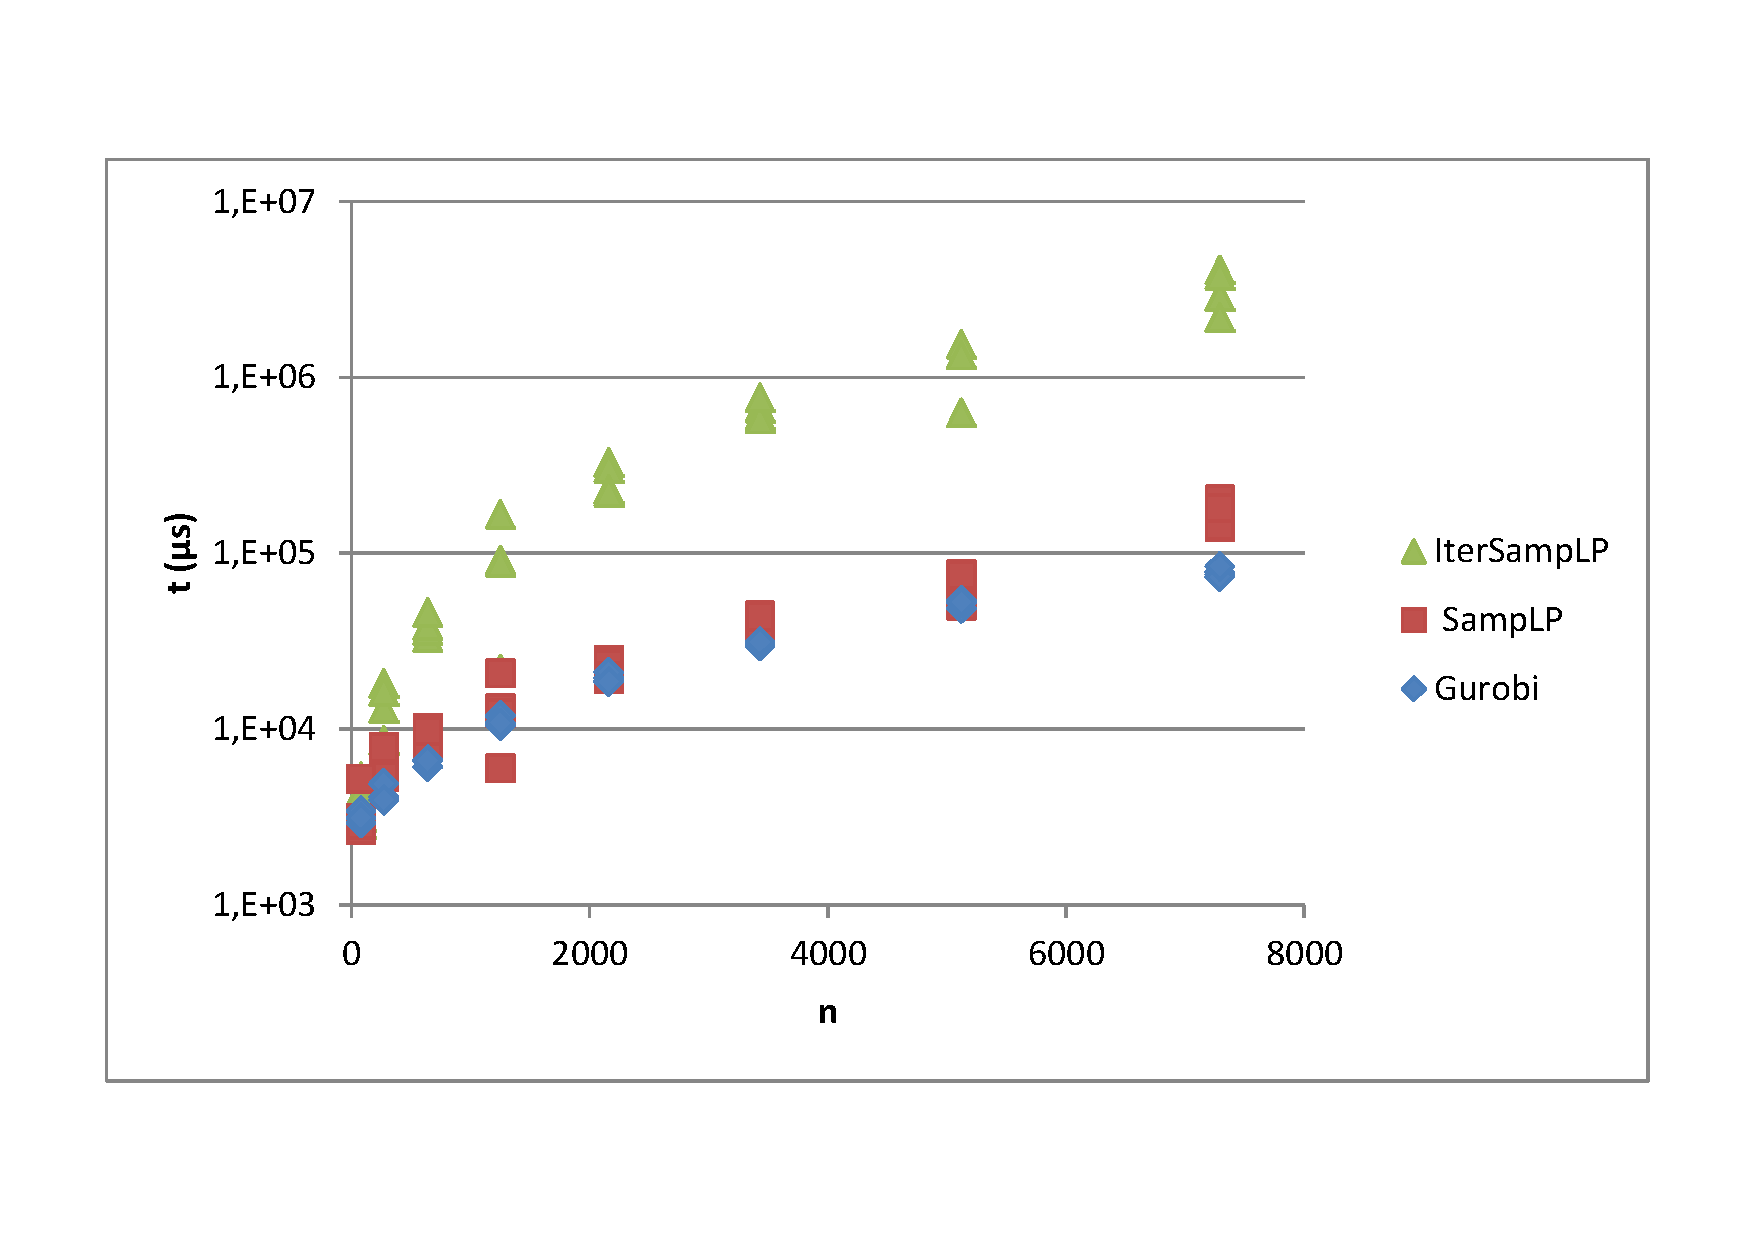
\includegraphics[width=\columnwidth]{../Results/gurobi_runtime.pdf}
\caption{Runtime results for Gurobi, SampLP and IterSampLP on the randomly generated problems. SampLP and IterSampLP use Gurobi instead of Simplex for obtaining an optimal solution}
\label{fig:gurobiruntime}
\end{figure}

\section{Conclusions}
The performance of three algorithms, among which two randomized, was tested on linear programming problem instances. The randomized algorithms that were tested,\\ SampLP and IterSampLP, were specifically designed to perform better on problem instances with small dimension. In the performance analysis this was indeed the case for SampLP. The deterministic algorithm Simplex was well out performed by SampLP. For some instances SampLP required in average only 3\% of the running time of Simplex to solve a problem. With smaller dimensions the gain was less significant, caused by the larger setup cost. Although SampLP performed much better than the tested Simplex implementation, it did not perform better than the commercial linear programming solver Gurobi. \\
IterSampLP did not out perform Simplex. When the runtime bound of IterSampLP is considered, this can be understood. The test cases that were generated for the analysis were too small to make use of this sophisticated algorithm. To be able to run bigger problem instances that might show the benefit of IterSampLP, better test equipment is required with more memory and computation power. \\
In this analysis the number of constraints was dependent on dimension of a problem. For better analysis these two values can be chosen separately (as long as the dimension is relatively small). Another suggestion is to generate random problems from a problem domain, instead of totally random. By generating problems from a specific domain, the runtime analysis might be more useful.

\bibliographystyle{abbrv}
\bibliography{sigproc}  % sigproc.bib is the name of the Bibliography in this case
\balancecolumns

\appendix
\begin{table}[h!]
\label{tab:miplibresults}
\caption{Runtime results for SimplexApache on instances of MIPLIB 2010 \cite{KochEtAl2011}}
\begin{tabularx}{\columnwidth}{|X|r|r|r|}
\hline
Problem Name     & $n$  & $d$   & $t$ (ms) \\ \hline
30n20b8          & 576  & 18,866 & 3,641   \\ \hline
50v-10           & 233  & 2,196  & 3,666   \\ \hline
acc-tight4       & 3,285 & 4,608  & 174,289 \\ \hline
acc-tight5       & 3,052 & 4,114  & 160,245 \\ \hline
acc-tight6       & 3,047 & 4,105  & 98,612  \\ \hline
beasleyC3        & 1,750 & 3,750  & 182,036 \\ \hline
bnatt400         & 5,614 & 3,600 & Stopped after 3h40m \\ \hline
cov1075          & 637  & 757   & 64,453  \\ \hline
enlight13        & 169  & 338   & 36     \\ \hline
enlight14        & 196  & 392   & 17     \\ \hline
enlight15        & 225  & 450   & 21     \\ \hline
enlight16        & 256  & 512   & 22     \\ \hline
enlight9         & 81   & 162   & 3      \\ \hline
ex1010-pi		 & 1,468 & 25,200 & Stopped after 2h50m \\ \hline
g200x740i        & 940  & 2,220  & 41,186  \\ \hline
ger50\_17\_trans & 499  & 22,641 & 128,743 \\ \hline
\end{tabularx}
\end{table}

\begin{table*}
\label{tab:relativeresults}
\centering
\caption{The runtime results (in microseconds) for SimplexApache, SampLP and IterSampLP on randomly generated linear programming problems with $d$ ranging from $2$ to $9$ and $n = 10d^3$. The runtime is an average over $100$ repetitions. A distinction is made between total runtime and the time that Simplex is running.}
\begin{tabular}{|l|l|l|l|l|l|l|l|} 
\hline
\#       & n    & d & SimplexApache & SampLP total & SampLP Simplex & IterSampLP total & IterSampLP Simplex \\ \hline
1        & 80   & 2 & 31                                                       & 25           & 10             & 127              & 13                 \\ \hline
2        & 80   & 2 & 106                                                      & 57           & 30             & 255              & 54                 \\ \hline
3        & 80   & 2 & 31                                                       & 25           & 9              & 135              & 14                 \\ \hline
4        & 80   & 2 & 31                                                       & 25           & 10             & 128              & 14                 \\ \hline
1        & 270  & 3 & 3518                                                     & 843          & 482            & 6767             & 1663               \\ \hline
2        & 270  & 3 & 2498                                                     & 627          & 314            & 4419             & 773                \\ \hline
3        & 270  & 3 & 1249                                                     & 449          & 189            & 2677             & 404                \\ \hline
4        & 270  & 3 & 2591                                                     & 681          & 353            & 5213             & 958                \\ \hline
1        & 640  & 4 & 24974                                                    & 3044         & 1815           & 27322            & 4874               \\ \hline
2        & 640  & 4 & 23685                                                    & 2223         & 1317           & 19794            & 3663               \\ \hline
3        & 640  & 4 & 12578                                                    & 2169         & 1250           & 18999            & 3526               \\ \hline
4        & 640  & 4 & 17826                                                    & 2374         & 1348           & 25389            & 4220               \\ \hline
1        & 1250 & 5 & 91605                                                    & 8571         & 3663           & 93396            & 8672               \\ \hline
2        & 1250 & 5 & 190610                                                   & 17437        & 10941          & 189220           & 38456              \\ \hline
3        & 1250 & 5 & 5599                                                     & 2080         & 181            & 17335            & 234                \\ \hline
4        & 1250 & 5 & 59826                                                    & 6676         & 2950           & 75248            & 8101               \\ \hline
1        & 2160 & 6 & 266887                                                   & 24334        & 13178          & 301377           & 43118              \\ \hline
2        & 2160 & 6 & 269059                                                   & 24017        & 13366          & 291398           & 45011              \\ \hline
3        & 2160 & 6 & 434566                                                   & 21049        & 11186          & 231637           & 25728              \\ \hline
4        & 2160 & 6 & 182747                                                   & 17205        & 8382           & 192605           & 22020              \\ \hline
1        & 3430 & 7 & 1402486                                                  & 56464        & 31761          & 650137           & 86166              \\ \hline
2        & 3430 & 7 & 805804                                                   & 57138        & 29486          & 685525           & 85931              \\ \hline
3        & 3430 & 7 & 1209336                                                  & 55658        & 27997          & 753164           & 86389              \\ \hline
4        & 3430 & 7 & 1349811                                                  & 67305        & 35871          & 950145           & 130263             \\ \hline
1        & 5120 & 8 & 2087614                                                  & 86721        & 32143          & 1428837          & 130015             \\ \hline
2        & 5120 & 8 & 2891915                                                  & 87656        & 36512          & 1643975          & 171009             \\ \hline
3        & 5120 & 8 & 1170917                                                  & 71039        & 28429          & 797186           & 68344              \\ \hline
4        & 5120 & 8 & 1545349                                                  & 78305        & 23893          & 1470287          & 101232             \\ \hline
1        & 7290 & 9 & 8944001                                                  & 252987       & 95365          & 5591116          & 751477             \\ \hline
2        & 7290 & 9 & 3770595                                                  & 171645       & 31653          & 4177553          & 267840             \\ \hline
3        & 7290 & 9 & 2190897                                                  & 171699       & 28134          & 3349625          & 210678             \\ \hline
4        & 7290 & 9 & 4572966                                                  & 201903       & 45554          & 4859949          & 348285             \\ \hline
\end{tabular}
\end{table*}


\end{document}
